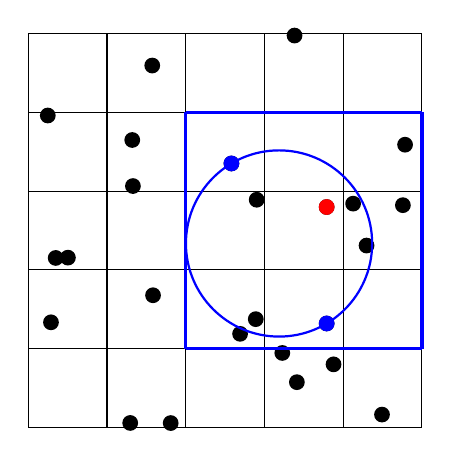
\begin{tikzpicture}
    \foreach \x in {0,1,...,5}{
        \draw (0,\x) -- (5,\x);
        \draw (\x,0) -- (\x,5);
    }
    %random numbers generated by Python
    \foreach \x / \y in {0.28897762565/1.33479488842, 1.29507843519/0.0567389232558, 1.32094528703/3.65045643132, 2.90131976409/2.89143039453, 3.38227004393/4.97678250754, 4.78587153595/3.59043085053, 4.49289684902/0.16312339617, 2.88976245038/1.37508072608, 0.503908610931/2.15612491084, 4.29648323686/2.30979809325, 1.57506933975/4.5958939884, 3.41193951077/0.574638720997, 1.58494426782/1.67834825887, 3.87742721851/0.800878920581, 0.34861369265/2.15217676901, 3.78999774171/1.31996000053, 3.22671310651/0.945568165194, 2.58060642147/3.3521091272, 1.8091306587/0.055518765505, 4.12621981945/2.84187520295, 2.69064049175/1.18843544815, 0.248568008024/3.96126629448, 1.32959523341/3.0654517407, 4.7582022563/2.8223407318, 3.78979061396/2.79890572216}{
        \fill (\x, \y) circle(0.1);
    }
    %~ 2.58060642147/3.3521091272
    %~ 3.78999774171/1.31996000053
    \def\xa{2.58060642147}
    \def\ya{3.3521091272}
    \def\xb{3.78999774171}
    \def\yb{1.31996000053}
    \def\x{3.1853020815900002}
    \def\y{2.3360345638649997}
    \def\d{1.1823977163477497}
    \fill[blue] (\xa,\ya) circle(0.1);
    \fill[blue] (\xb,\yb) circle(0.1);
    \fill[red] (3.78979061396,2.79890572216) circle(0.1);
    \draw[blue,very thick] (2,1) -- (5,1);
    \draw[blue,very thick] (2,4) -- (5,4);
    \draw[blue,very thick] (2,1) -- (2,4);
    \draw[blue,very thick] (5,1) -- (5,4);
    \draw[blue,thick] (\x, \y) circle(\d);
\end{tikzpicture}
